\section{Operating Modes}
The SPI core's versatility is exemplified by its ability to operate in both master and slave modes. Each mode offers distinct functionalities and configurations to cater to diverse system requirements.

\subsection{Master Mode}
In master mode, the SPI core assumes control over the communication process. It is responsible for generating the serial clock (SCK) and managing the Slave Select (SS) lines to initiate and terminate communication with slave devices.

\subsubsection{Normal Mode}
Operating in normal mode without buffering involves the following characteristics:

\begin{itemize}
    \item \textbf{Immediate Transmission:} Data transmission begins as soon as data is written to the Data Register (\texttt{DATA}).
    \item \textbf{Single-Buffered Transmission:} The SPI core uses a single buffer for transmission, meaning only one byte can be sent at a time.
    \item \textbf{Double-Buffered Reception:} Reception is handled using a double buffer, allowing for more efficient data handling without data loss.
    \item \textbf{Write Collision Detection:} If an attempt is made to write to \texttt{DATA} before the current transmission completes, the Write Collision flag (\texttt{WRCOL}) is set, indicating a collision has occurred.
\end{itemize}

\subsubsection{Buffer Mode}
Enabling buffer mode introduces additional buffering capabilities, enhancing data handling efficiency:

\begin{itemize}
    \item \textbf{Double-Buffered Transmission:} Allows two bytes to be buffered for transmission, enabling continuous data flow without waiting for the previous transmission to complete.
    \item \textbf{Triple-Buffered Reception:} Reception is managed using three buffers, providing ample space to handle incoming data without overflow.
    \item \textbf{Interrupt-Driven Operations:} Buffer mode facilitates the use of interrupts for efficient data handling. The Data Register Empty Interrupt Flag (\texttt{DREIF}) can be used to determine when \texttt{DATA} is ready to accept new data.
    \item \textbf{Enhanced Throughput:} By allowing multiple bytes to be buffered, buffer mode significantly increases the data throughput, making it suitable for high-speed data transfers.
\end{itemize}

% Master Mode Timing Diagram
\begin{figure}[H]
    \centering
    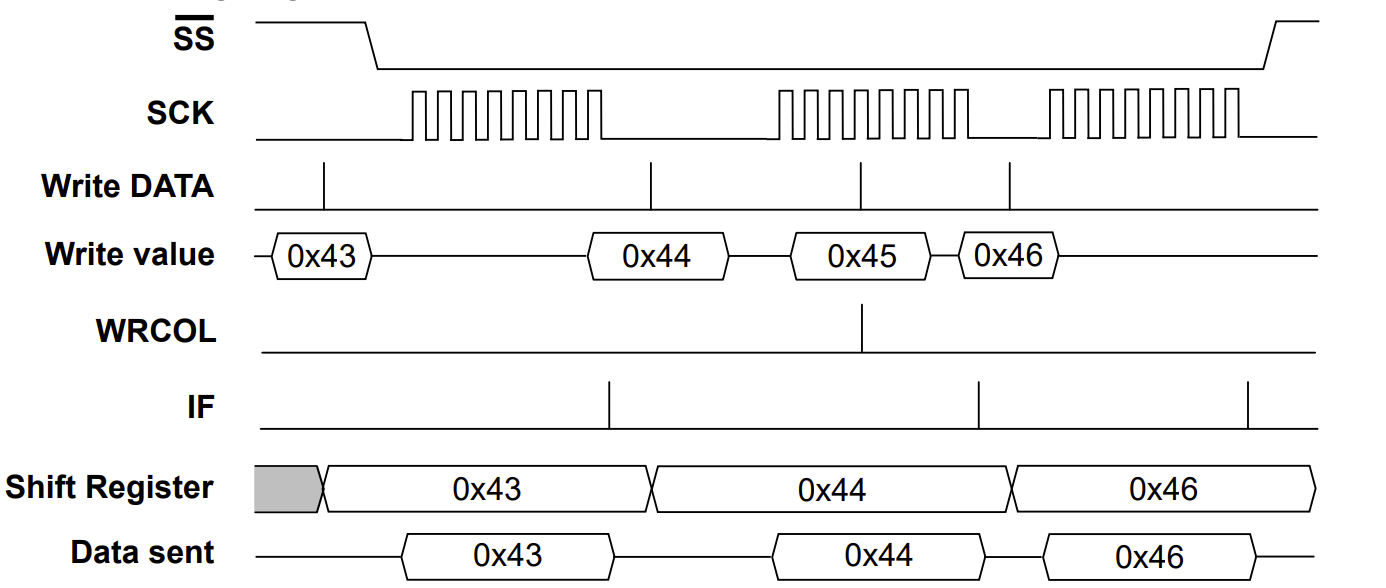
\includegraphics[width=0.85\textwidth]{images/spi_master_timing.png}
    \caption{Master Mode Timing Diagram}
    \label{fig:spi_master_timing}
\end{figure}

\subsubsection{Normal Mode}
In normal mode without buffering:

\begin{itemize}
    \item \textbf{Transmission starts immediately after writing to \texttt{DATA}.}
    \item \textbf{The core is single-buffered for transmission and double-buffered for reception.}
    \item \textbf{The Write Collision flag (\texttt{WRCOL}) is set if \texttt{DATA} is written before a transmission completes.}
\end{itemize}

\subsubsection{Buffer Mode}
Enabling buffer mode provides additional buffering:

\begin{itemize}
    \item \textbf{Double-buffered transmission and triple-buffered reception.}
    \item \textbf{Allows writing to \texttt{DATA} while a transmission is ongoing.}
    \item \textbf{Use the Data Register Empty Interrupt Flag (\texttt{DREIF}) to check if \texttt{DATA} can be written.}
\end{itemize}

% Buffer Mode Diagram
\begin{figure}[H]
    \centering
    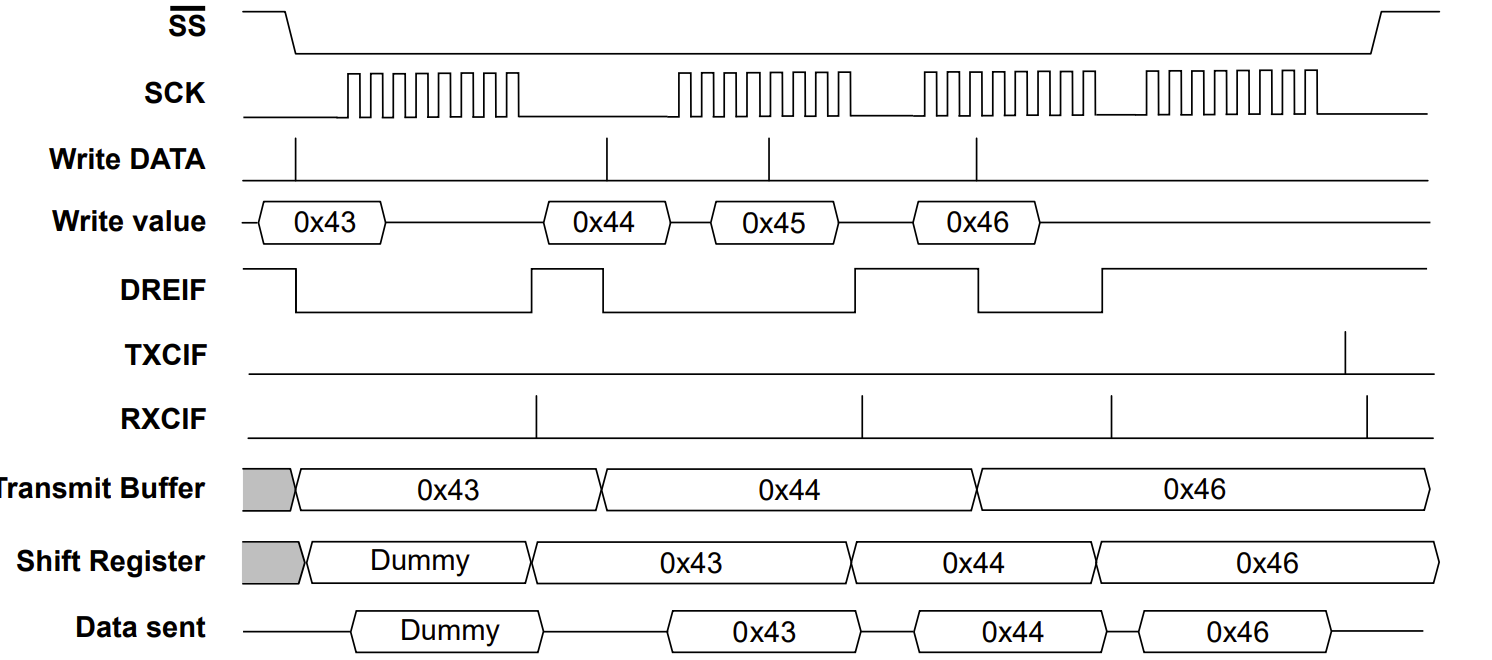
\includegraphics[width=0.85\textwidth]{images/spi_buffer_mode.png}
    \caption{SPI Buffer Mode Operation}
    \label{fig:spi_buffer_mode}
\end{figure}

\subsection{Slave Mode}
In slave mode, the SPI core operates passively, awaiting instructions from the master device. It does not generate the clock signal but instead responds to the master's SCK and SS signals.

\subsubsection{Normal Mode}
Operating in normal mode without buffering involves the following characteristics:

\begin{itemize}
    \item \textbf{Initiated by Master:} Transmission and reception are controlled by the master device, which dictates when data transfers occur.
    \item \textbf{Data Preparation:} Data must be written to the Data Register (\texttt{DATA}) before the master initiates a transfer. Failure to do so can result in incomplete or corrupted data transmission.
    \item \textbf{Write Collision Detection:} Similar to master mode, if \texttt{DATA} is written during an ongoing transfer, the Write Collision flag (\texttt{WRCOL}) is set, indicating a collision.
\end{itemize}

\subsubsection{Buffer Mode}
Buffer mode in slave operation offers enhanced data handling capabilities:

\begin{itemize}
    \item \textbf{Pre-Buffered Transmission:} Allows the slave to prepare multiple bytes of data in advance, ensuring seamless data transmission when the master initiates a transfer.
    \item \textbf{Graceful Overrun Handling:} Buffer mode can detect and manage data overruns, preventing data loss and maintaining system stability.
    \item \textbf{Configurable Buffer Behavior:} The Buffer Mode Wait for Receive (\texttt{BUFWR}) bit in \texttt{CTRLB} allows configuration of how the buffer behaves during data reception, enabling flexible data handling strategies.
\end{itemize}

% Slave Mode Timing Diagram
\begin{figure}[H]
    \centering
    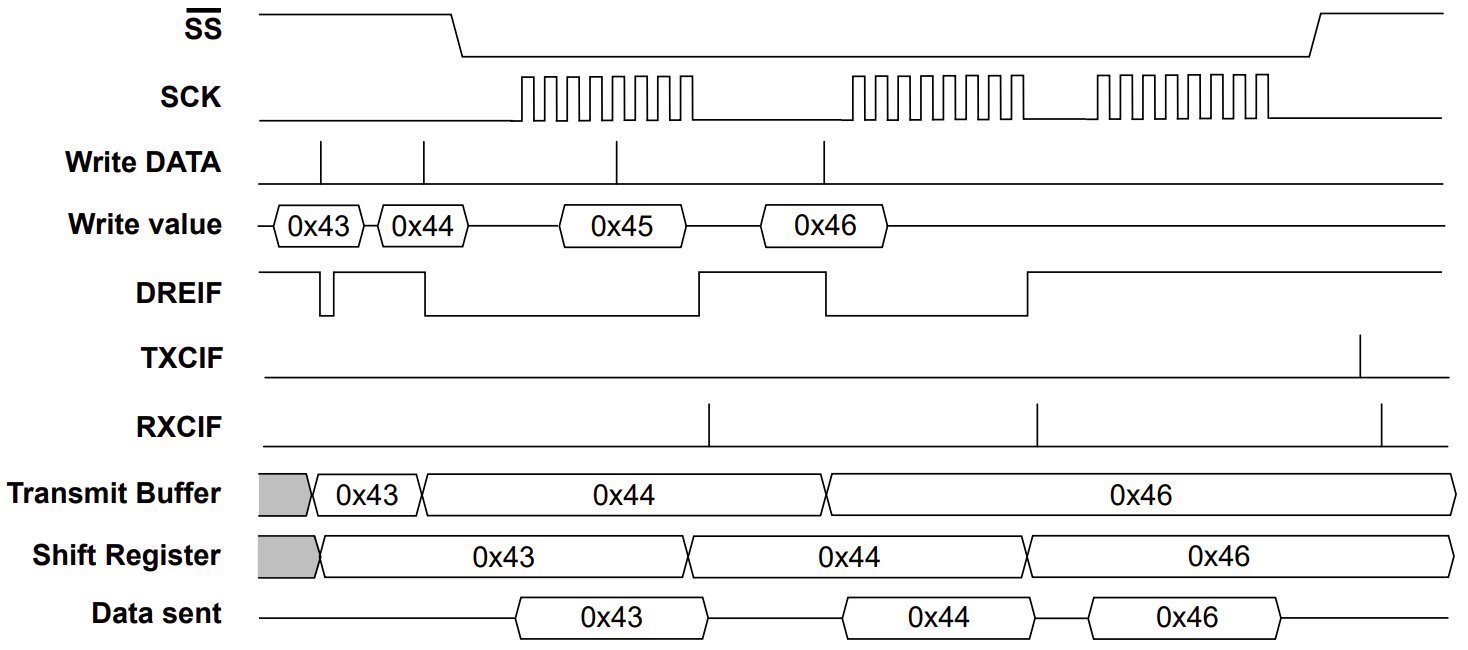
\includegraphics[width=0.85\textwidth]{images/spi_slave_timing.png}
    \caption{Slave Mode Timing Diagram}
    \label{fig:spi_slave_timing}
\end{figure}

\subsubsection{Normal Mode}
In normal mode:

\begin{itemize}
    \item \textbf{Transmission begins when SS is low and SCK pulses are received.}
    \item \textbf{Data must be written to \texttt{DATA} before the master initiates a transfer.}
    \item \textbf{The Write Collision flag (\texttt{WRCOL}) is set if \texttt{DATA} is written during an ongoing transfer.}
\end{itemize}

\subsubsection{Buffer Mode}
Buffer mode in slave operation allows for:

\begin{itemize}
    \item \textbf{Preparing data in advance for transmission.}
    \item \textbf{Handling data overruns more gracefully.}
    \item \textbf{Configurable behavior using the Buffer Mode Wait for Receive (\texttt{BUFWR}) bit.}
\end{itemize}

% % Slave Buffer Mode Diagram
% \begin{figure}[H]
%     \centering
%     \includegraphics[width=0.85\textwidth]{images/spi_slave_buffer_mode.png}
%     \caption{Slave Buffer Mode Operation}
%     \label{fig:spi_slave_buffer_mode}
% \end{figure}

\subsection{Data Transfer Modes}
The SPI protocol defines four distinct data transfer modes, each determined by the Clock Polarity (CPOL) and Clock Phase (CPHA). These modes dictate the timing relationship between the clock signal and data signals, ensuring synchronized and accurate data transmission.

\begin{table}[H]
    \centering
    \caption{SPI Data Transfer Modes}
    \begin{tabular}{@{}ccc@{}}
        \toprule
        \textbf{Mode} & \textbf{CPOL} & \textbf{CPHA} \\ \midrule
        0 & 0 & 0 \\
        1 & 0 & 1 \\
        2 & 1 & 0 \\
        3 & 1 & 1 \\ \bottomrule
    \end{tabular}
    \label{tab:spi_modes}
\end{table}

\begin{itemize}
    \item \textbf{Mode 0 (CPOL=0, CPHA=0):} 
    \begin{itemize}
        \item \textbf{Clock Polarity (CPOL):} The clock signal (SCK) is low when idle.
        \item \textbf{Clock Phase (CPHA):} Data is sampled on the leading (rising) edge of the clock.
        \item \textbf{Description:} Data is set up on the trailing edge and sampled on the leading edge, ensuring data stability before sampling.
    \end{itemize}
     
    \item \textbf{Mode 1 (CPOL=0, CPHA=1):}
    \begin{itemize}
        \item \textbf{Clock Polarity (CPOL):} The clock signal (SCK) is low when idle.
        \item \textbf{Clock Phase (CPHA):} Data is sampled on the trailing (falling) edge of the clock.
        \item \textbf{Description:} Data is set up on the leading edge and sampled on the trailing edge, providing flexibility in data timing.
    \end{itemize}
    
    \item \textbf{Mode 2 (CPOL=1, CPHA=0):}
    \begin{itemize}
        \item \textbf{Clock Polarity (CPOL):} The clock signal (SCK) is high when idle.
        \item \textbf{Clock Phase (CPHA):} Data is sampled on the leading (falling) edge of the clock.
        \item \textbf{Description:} Data is set up on the trailing edge and sampled on the leading edge, suitable for systems where a high idle clock state is preferred.
    \end{itemize}
    
    \item \textbf{Mode 3 (CPOL=1, CPHA=1):}
    \begin{itemize}
        \item \textbf{Clock Polarity (CPOL):} The clock signal (SCK) is high when idle.
        \item \textbf{Clock Phase (CPHA):} Data is sampled on the trailing (rising) edge of the clock.
        \item \textbf{Description:} Data is set up on the leading edge and sampled on the trailing edge, allowing for alternate data sampling strategies.
    \end{itemize}
\end{itemize}

% Data Transfer Modes Timing Diagrams
\begin{figure}[H]
    \centering
    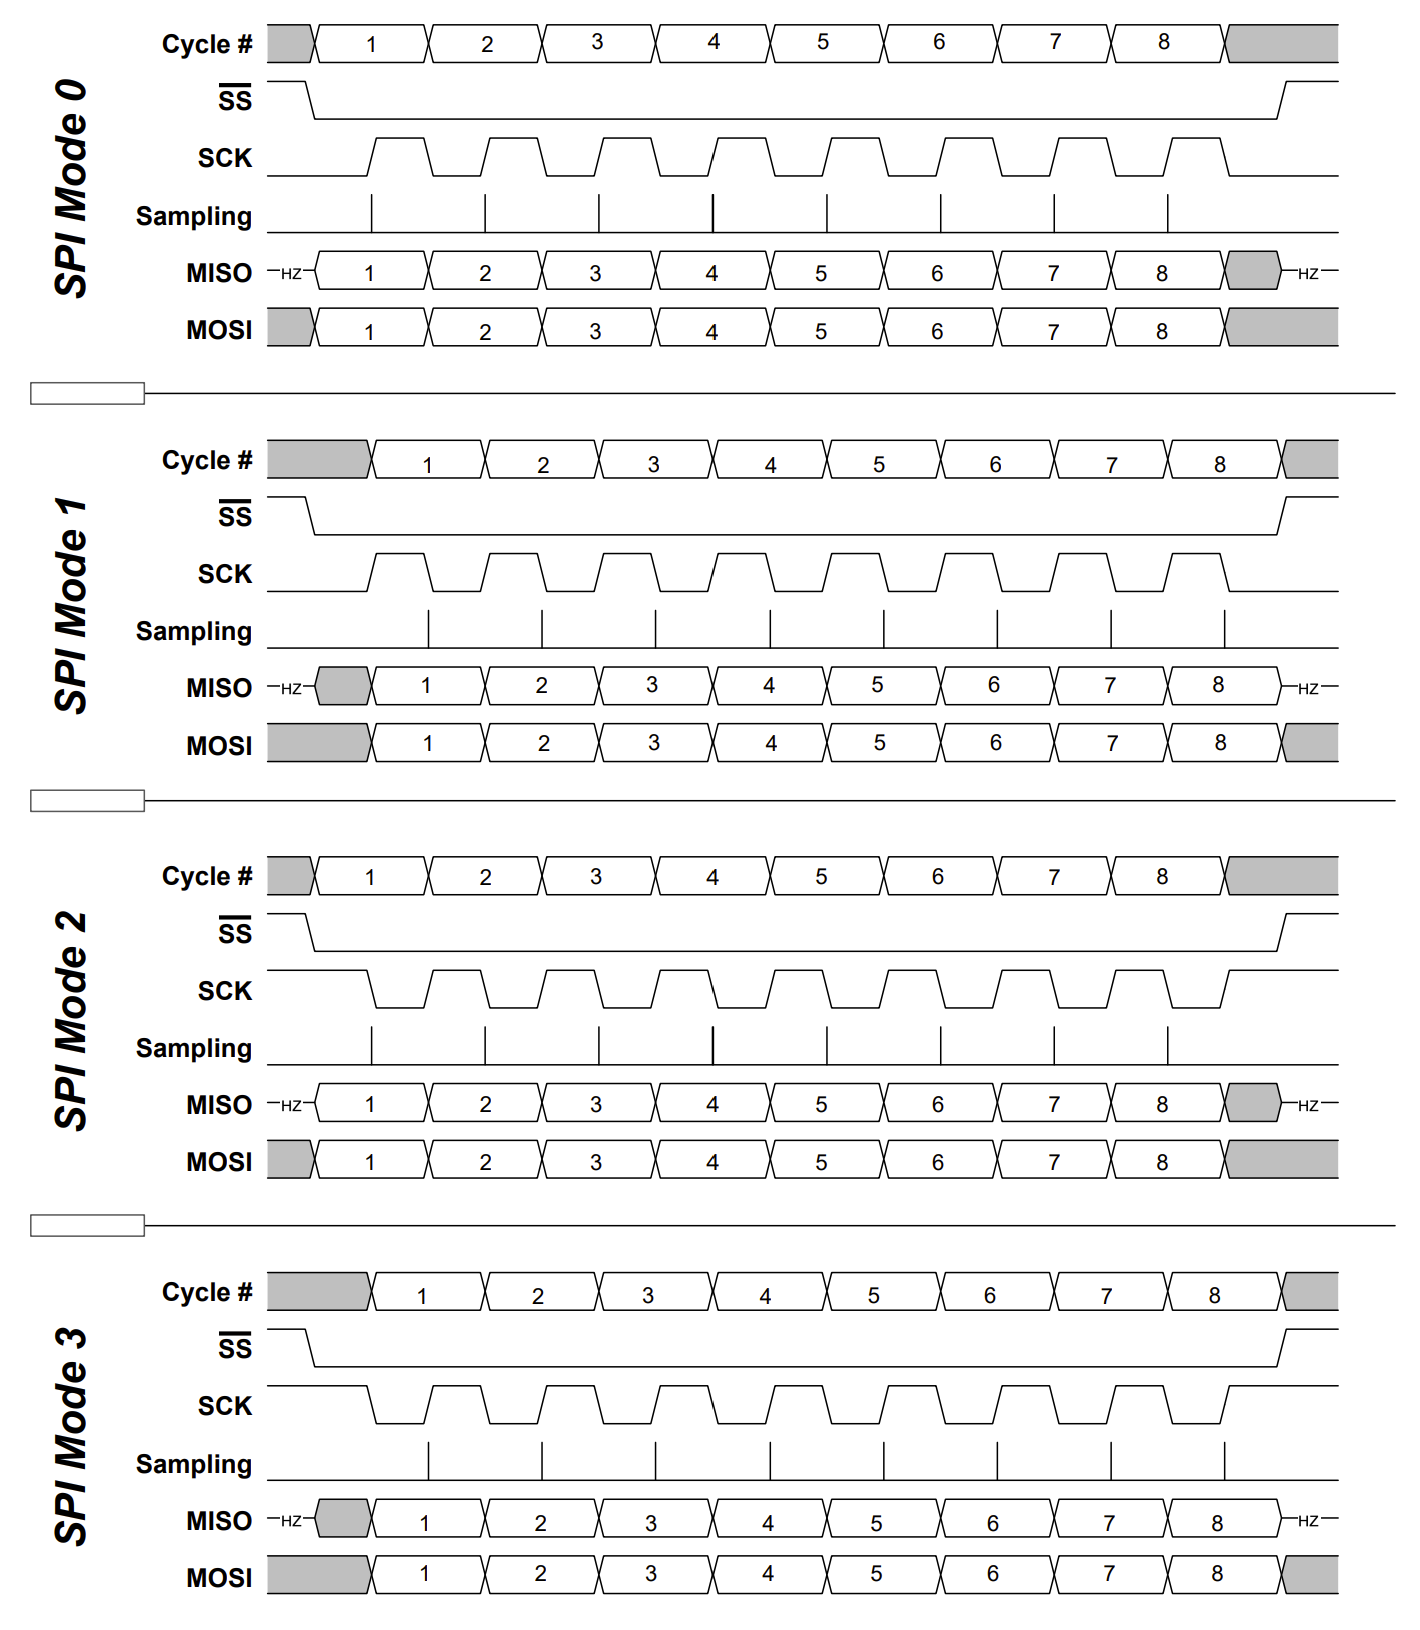
\includegraphics[width=0.9\textwidth]{images/spi_data_modes.png}
    \caption{SPI Data Transfer Modes Timing Diagrams}
    \label{fig:spi_data_modes}
\end{figure}